\section{Motorization: microcontrollers}

\subsection{ESP32}
ESP32 is a series of low-cost, low-power system on a chip microcontroller with integrated Wi-Fi and dual-mode Bluetooth.
We've bought the ESP32 D1 R32, the one in figure \ref{fig:esp32}, for better attaching the motor using the CNC shield V3 (which is briefly explained in the following).

We decided to follow the "Wemos R32 and CNC V3" OnStep project (at \url{https://onstep.groups.io/g/main/wiki/19670}).
OnStep is an open source software providing the control of four stepper motors (RA, DEC, focuser and rotator for astrophotography), weather sensor handling, Wi-Fi and Bluetooth connection, polar alignment and other nice features.

\begin{minipage}
    {.4\textwidth}
    \centering
    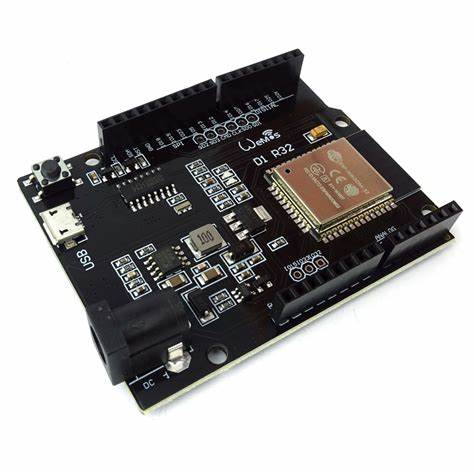
\includegraphics[scale=0.28]{esp32_d1_r32.jpg}
    \captionof{figure}{ESP32 D1 R32 picture.}
    \label{fig:esp32}
\end{minipage}

\subsection{CNC Shield V3}
To better optimize space and wires connections, we have bought a CNC Shield V3 (aka CNC3), see figure \ref{fig:cnc3}.
\begin{minipage}
    {0.5\textwidth}
    \centering
    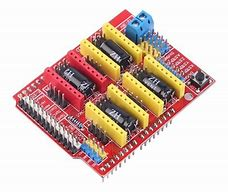
\includegraphics[scale=0.5]{CNC3.jpg}
    \captionof{figure}{CNC3 Shield V3.}
    \label{fig:cnc3}
\end{minipage}
It is a shield built to be used for 3D printers.
The shield is attached directly above the ESP32.
It has four slots, each one can host a motor driver, thus using this shield there can be handled four stepper motors: RA and DEC motors, first focuser and photography rotator or second focuser.

This shield can be "manipulated" to obtain better performances.

\subsection{CNC3 modifications}
\hl{aggiungere qui}
\subsubsection{Microsteps control}
\hl{aggiungere qui}

\subsubsection{Microsteps gotos control}
\hl{aggiungere qui}

\subsection{Motor drivers}
A stepper motors works only with a driver chip that controls the motor movements.
Three types of drivers have been used during the configuration of the setup.
\begin{enumerate}
    \item DRV8825;
    \item TMC2209;
    \item TMC2208.
\end{enumerate}

In each driver the right amount of current is set, otherwise the stepper motor could work improperly.
This current depends on the stepper motor current per phase parameter.
Typically, drivers have a tunable screw for the tension \(V_{ref}\).
For each type of driver, the formula to calculate the tension \(V_{ref}\) depending on the current/phase are different.\footnote{See \url{https://all3dp.com/2/vref-calculator-tmc2209-tmc2208-a4988/} for more details.}

The procedure is the following:
\begin{itemize}
    \item rotate the screw in the counter clock direction;
    \item using a multimeter, check that the tension is zero;
    \item slightly rotate the screw until the tension is the desired one.
\end{itemize}
We recommend reducing the theoretical value by a 10\%-30\% to prevent motor dangers.

\subsubsection{DRV8825}
For these drivers the tension to be set is roughly the half of the value of the nominal current/phase of the motor.
For example, if the motor has a current/phase \(1\)A, the tension would be \(0.5\)V.

\begin{minipage}
    {.4\textwidth}
    \begin{tabular}{cc}
        Current phaser (A) & Current (A) \\
        \hline
        0.90 & 0.45 \\
        2.00 & 0.90             
    \end{tabular}
    \captionof{table}{DRV8828 drivers setup current. Note that we have set a value smaller than the one calculated to prevent motor to break.}
    \label{tab:drivers_curr}
\end{minipage} 

\subsubsection{TMC2208 and TMC2209}
For these drivers the tension value is roughly the same of the current/phase value, \textit{e.g.} if \(I=1\)A the tension would be \(V_{ref}=1\)V.
Be aware that the TMC2208 has a maximum current output of 1.2A.

The calculation is 
\[\frac{I}{\sqrt{2}}=\frac{325mV}{110m\Omega+20m\Omega}\cdot\frac{1}{\sqrt{2}}\cdot\frac{V_{ref}}{2.5V}\Rightarrow V_{ref} = I \cdot 1\Omega.\]
Remember to reduce to value by a 10\%-30\%.

\begin{minipage}
    {.4\textwidth}
    \begin{tabular}{ccc}
       Driver & Current/phase (A) & Current (A) \\
        \hline
       TMC2208 & 0.90 & 0.81 \\
       TMC2208 &  2.00 & 1.63 \\                
       TMC2209 (focuser) &  0.67 & 0.50                
    \end{tabular}
    \captionof{table}{DRV8825 drivers setup current. Note that we have set a value smaller than the one calculated to prevent motor to break.}
    \label{tab:drivers_curr}
\end{minipage} 

\subsection{Power supply}
The power supply is provided by a 19V 5A power supply as in table \ref{tab:power_supply}.

\begin{minipage}
    {.4\textwidth}
    \begin{tabular}{cc}
         voltage output (V) & current output (A) \\
         \hline
        19.3 & 4.74 \\
    \end{tabular}
    \captionof{table}{Nominal tension and current outputs of the power supply.}
    \label{tab:power_supply}
\end{minipage}

For our initial purposes it was enough, indeed 5A are enough to feed quite well two stepper motors and a poor electronics.
A rough estimation poses 1.8A for DEC motor, 0.9A for RA motor and few milliampéres for the ESP32. 
The reader is strongly encouraged to check the total current its circuit needs before buying a power supply.

\subsection{Sensors: Wi-Fi connection, Real time clock (RTC) and weather sensor (BMP280)}
An ESP8688 WeMos D1 mini is connected to the CNC3 as shown in \url{https://onstep.groups.io/g/main/wiki/19670}.

This OnStep has a software addon called the Smart Web Server (SWS) which provides WiFi or Ethernet connections over IP.
Many devices support this type of connection including cell-phones, tablets, laptop/desktop computers, etc.
Using this library, it is possible to use programs such as Stellarium via ASCOM drivers provided by the OnStep project \url{http://www.stellarjourney.com/index.php?r=site/software_telescope}.